\documentclass{beamer}

\usepackage[utf8x]{inputenc}
\usepackage{graphicx}
\usepackage{default}
\usetheme{Dresden}
\usecolortheme{sidebartab}

\title[HCI Studio]{HCI Studio}
\author[Vikoler]{Stefan Vikoler}
\institute{University of Salzburg}
\date[19. 11. 2014]{19. November 2014}

\begin{document}

\frame{
  \titlepage
}
\frame{
  \frametitle{Aufgabenstellung}
    \begin{itemize}
      \item Think about 3 Ideas about alternative interaction konzepts regarding the steering wheel of a car.\\ \ \\
      \item Touch the sound (Speak with the sound)
      \item Think reverse
      \item Tune your car\\ \ \\
      \item Rat race
    \end{itemize}
}
\frame{
  \frametitle{Touch the sound}
    \begin{itemize}
      \item Interface:
      \begin{itemize}
	\item Touch interface on the front side of the steering wheel\\
	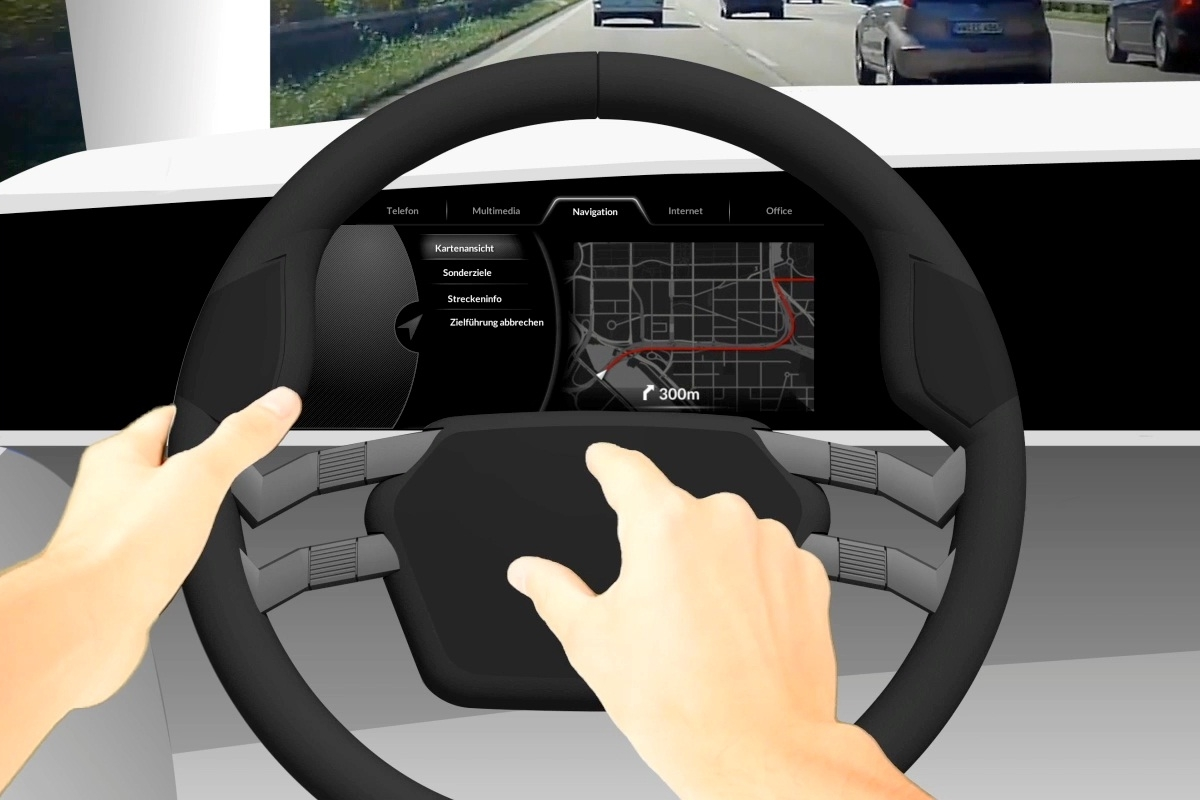
\includegraphics[width=150px]{touch.jpg}\\
	{\tiny \textit{http://blog.audi.de/}}
      \end{itemize}
    \end{itemize}
}
\frame{
  \frametitle{Touch the sound}
    \begin{itemize}
      \item Functionality:
      \begin{itemize}
	\item Control and interact with the radio with different signs on the touch screen
	\item For example letters or digits
      \end{itemize}
      \item Speak with the sound:
      \begin{itemize}
	\item Alternatively someone can also control the radio by simple voice control
      \end{itemize}
    \end{itemize}
}
\frame{
  \frametitle{Think reverse}
    \begin{itemize}
      \item Interface:
      \begin{itemize}
	\item Yoke like on a airplane\\
	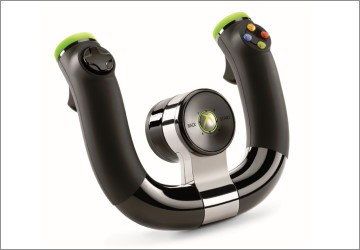
\includegraphics[width=150px]{reverse1.jpg}\\
	{\tiny \textit{http://www.xboxaktuell.de/}}
      \end{itemize}
    \end{itemize}
}
\frame{
  \frametitle{Think reverse}
    \begin{itemize}
      \item Interface:
      \begin{itemize}
	\item Two pedals like in a car\\
	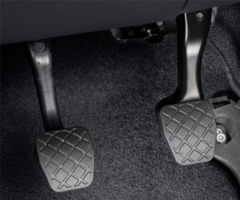
\includegraphics[width=150px]{reverse2.jpg}\\
	{\tiny \textit{http://www.consumerreports.org/}}
      \end{itemize}
    \end{itemize}
}
\frame{
  \frametitle{Think reverse}
    \begin{itemize}
      \item Functionality:
      \begin{itemize}
	\item Control the speed of the car by pushing and pulling the yoke
	\begin{itemize}
	  \item push $\rightarrow$ accelerate
	  \item pull $\rightarrow$ slow down / break
	\end{itemize}
	\item Control the direction of the car by stepping on the left or right pedal
	\begin{itemize}
	  \item left pedal $\rightarrow$ turn left
	  \item right pedal $\rightarrow$ turn right
	\end{itemize}
      \end{itemize}
    \end{itemize}
}
\frame{
  \frametitle{Tune your car}
    \begin{itemize}
      \item Interface:
      \begin{itemize}
	\item Interface elements from a DJ console
	\begin{itemize}
	  \item buttons
	  \item slide-controls, ...
	\end{itemize}
	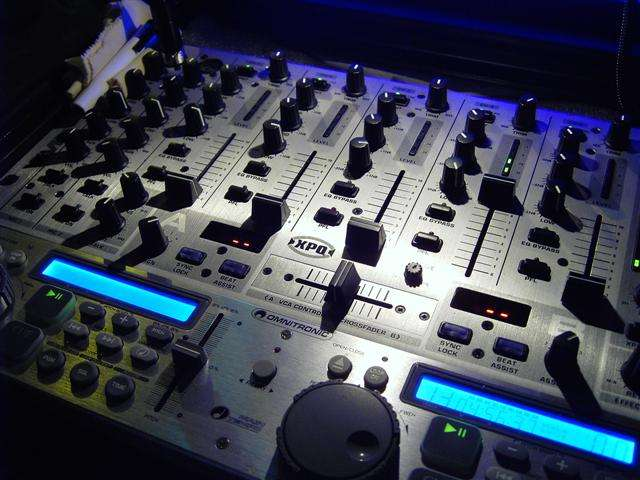
\includegraphics[width=150px]{tune.jpg}\\
	{\tiny \textit{http://dejavu.am}}
      \end{itemize}
    \end{itemize}
}
\frame{
  \frametitle{Tune your car}
    \begin{itemize}
      \item Functionality:
      \begin{itemize}
	\item Control the speed of the car with a horizontal slide-control
	\item Control the direction of the car with a vertical slide-control
	\item Control a lot of other elements like turning lights and wipers by buttons and switches
      \end{itemize}
    \end{itemize}
}
\frame{
  \frametitle{Rat race}
    \begin{itemize}
      \item Interface:
      \begin{itemize}
	\item Idea: rat race wheel for hamsters\\
	
\includegraphics[width=150px]{ratrace.png}\\
	{\tiny \textit{http://www.inboundsales.net/}}
      \end{itemize}
    \end{itemize}
}
\frame{
  \frametitle{Rat race}
    \begin{itemize}
      \item Interface:
      \begin{itemize}
	\item Solution: Walking Ball to be able to run in all possible directions\\
	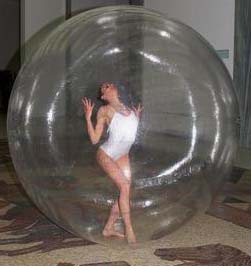
\includegraphics[width=120px]{walkingball.jpg}\\
	{\tiny \textit{http://inflatable.china-direct-buy.com/}}
      \end{itemize}
    \end{itemize}
}
\frame{
  \frametitle{Rat race}
    \begin{itemize}
      \item Functionality:
      \begin{itemize}
	\item Control the speed by simply running faster
	\item Control the direction by simply aiming to this direction
	\item Drive backwards by running backwards
	\item ...
      \end{itemize}
    \end{itemize}
}
\frame{
  \titlepage
}

\end{document}
